\section{N+1 view model}

N + 1 view modellen bruges til at beskrive software fra forskellige views. Modellen tager altid udgangspunkt i et use case view. Derefter er det op til udviklerholdet at bestemme hvor mange views der skal bruges for at beskrive systemet på tilstrækkelig vis. Til beskrivelse af dette system anvendes en 5 + 1 view model. På figur \ref{fig:5 + 1 view model} vises den anvendte model


\vspace{-5pt}
\begin{figure}[H]
	\centering
	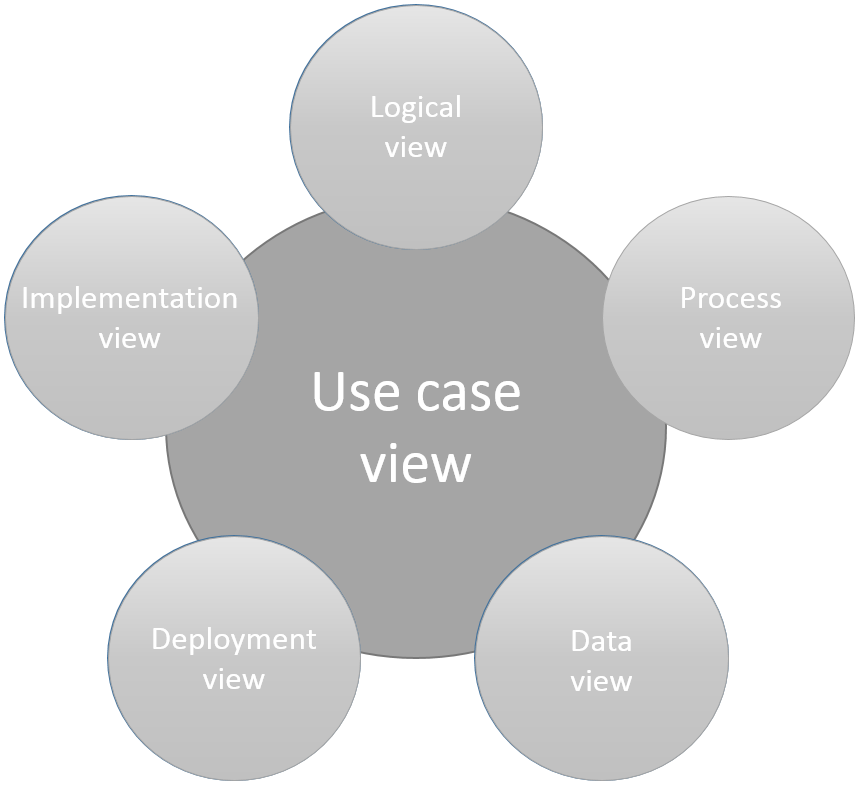
\includegraphics[width=0.7\textwidth]{Billeder/n+1}
	\vspace{0cm}
	\caption{5 + 1 view model}
	\label{fig:5 + 1 view model}
\end{figure}


\newpage

\subsection{View beskrivelser}

\textbf{Use case view}\\
Use case viewet består af use case diagrammer, som er udviklet ud fra bruges synspunkt og som bruges til at beskrive systemets forskellige brugsscenarier. Alle udarbejdede use case diagrammer forefindes i kravspecifikations dokumentet.

\textbf{Logical view}\\
Logical viewet består i udgangspunkt af følgende fire diagrammer: Designoverviewdiagrammer, sekvensdiagrammer, statemachines og klassediagrammer. Først laves designoverviewdiagrammer, dernæst udarbejdes sekvensdiagrammer som bruges til at beskrive det overordnede flow i systemet. Hvis det giver mening udarbejdes statemachines, som bruges til at vise hvilke states en given use case indeholder. Til sidst laves klassediagrammer og alle "aktive" klasser identificeres. 

\textbf{Process view}\\
Process viewet beskriver de forskellige processer/tråde i systemet og hvordan samspillet imellem disse er. Primært beskrives sammenspil mellem processer/tråde der kører sideløbende med hinanden.

\textbf{Data view}\\
I data viewet beskrives layout af data der gemmes og hvordan det lagres. Desuden beskrives hvordan data bevæger sig rundt i systemet og hvordan database tilgås. 

\textbf{Deployment view}\\
I deployment viewet kigges på systemets mest grundlæggende og overordnede klasser. Det beskrives hvilke forskellige softwareklasser der bruges i hver af de grundlæggende klasser. Desuden beskrives hvilke protokoller der er anvendt i systemet, fx. layout af meddelelser med header/start/stop.   

\textbf{Implementation view}\\
I løbet af et længere projekt forløb genereres altid en masse filer - i implementations viewet vises bla. hvilke filer systemet er bygget af, filstruktur og hvilken compiler der er benyttet. 
Målet med implemantations viewet er at gøre det muligt for udefrakommende at genoptage arbejde på projektet på et hvilket som helst tidspunkt.


